%%%%%%%%%%%%%%%%%%%%%%%%%%%%%%%%%%%%%%%%%%%%%%%%%%%%%%%%%%%%%%%%%%%%%%%%%
%% Linear Algebra -- course project report template, Autumn 2026
%% Ukrainian Catholic University, Faculty of Applied Sciences,
%% Data Science Master Programme
%%
%% The title page is adapted from a template by WikiBooks, distributed
%% by LaTeXTemplates.com under CC BY-NC-SA 3.0.
%%
%% HOW TO USE THIS TEMPLATE
%%   1. Fill in the block marked "FILL IN" below: the stage of the report,
%%      the title, the authors, the project card and the links.
%%   2. One file serves all three milestones. Keep working in the same
%%      file: interim report 1 grows into interim report 2, and that grows
%%      into the final report.
%%   3. Replace the grey guidance boxes with your own text. Before you
%%      submit, set \showguidefalse so that any box you forgot disappears.
%%   4. Do NOT change the font size, the paper size or the margins.
%%      Page limits are counted in this format.
%%   5. Compile with pdfLaTeX (the Overleaf default). The folder must
%%      contain UCU-Apps.png (the logo); the example figure uses an image
%%      shipped with every TeX distribution.
%%
%% PAGE LIMITS (counted automatically; see the end of the log file)
%%   Interim report 1: 2 pages; interim report 2: 4-5 pages, project card included.
%%   Final report: at most 10 pages from the abstract to the end of the
%%   Conclusion, figures and tables included. The title page, the
%%   references and the appendices are not counted.
%%%%%%%%%%%%%%%%%%%%%%%%%%%%%%%%%%%%%%%%%%%%%%%%%%%%%%%%%%%%%%%%%%%%%%%%%

\documentclass[11pt,a4paper]{article}

%----------------------------------------------------------------------
%  Page layout: do not change
%----------------------------------------------------------------------
\usepackage[a4paper,left=20mm,right=20mm,top=20mm,bottom=25mm,
            headheight=14pt,marginparwidth=16mm]{geometry}

%----------------------------------------------------------------------
%  Packages
%----------------------------------------------------------------------
\usepackage[english]{babel}
% T1 encoding only together with the scalable Latin Modern fonts
% (standard on Overleaf); otherwise fall back to the default encoding.
\IfFileExists{lmodern.sty}{\usepackage[T1]{fontenc}\usepackage{lmodern}}{}
\usepackage{microtype}
\usepackage{amsmath,amssymb,amsthm}
\usepackage{graphicx}
\usepackage{booktabs,tabularx}
\usepackage{caption,subcaption}
\usepackage[dvipsnames]{xcolor}
\usepackage{fancyhdr}
\usepackage{refcount}
\usepackage{listings}
\usepackage[ruled,vlined,linesnumbered]{algorithm2e}
% Margin notes are useful while drafting. Add the option "disable"
% before you submit, or simply delete your \todo{} commands.
\usepackage[colorinlistoftodos,textsize=scriptsize]{todonotes}
\usepackage[colorlinks=true,linkcolor=MidnightBlue,citecolor=MidnightBlue,
            urlcolor=MidnightBlue]{hyperref}   % load hyperref last

%%%%%%%%%%%%%%%%%%%%%%%%%%%%%%%%%%%%%%%%%%%%%%%%%%%%%%%%%%%%%%%%%%%%%%%%%
%%%%%%%%%%%%%%%%%%%%%%%%%%%%%%%%%%%%%%%%%%%%%%%%%%%%%%%%%%%%%%%%%%%%%%%%%
%%  FILL IN
%%%%%%%%%%%%%%%%%%%%%%%%%%%%%%%%%%%%%%%%%%%%%%%%%%%%%%%%%%%%%%%%%%%%%%%%%

% Stage of the report: 1 = interim report 1 (scoping memo),
%                      2 = interim report 2 (working baseline),
%                      3 = final report
\newcommand{\stage}{2}

\newcommand{\reporttitle}{Low-Rank Spectral Fingerprints for AI-Generated Music Detection}
\newcommand{\shorttitle}{Low-rank spectrograms for AI-music detection}
\newcommand{\reportauthors}{Iryna Matvieieva \quad Petro Mozil}

% Project card: one line each. Keep it consistent with your registration;
% if something has changed, update it here and say so in the report.
\newcommand{\carddomain}{Audio forensics / music provenance}
\newcommand{\cardmethod}{Log-magnitude STFT spectrograms; exact SVD per clip, randomized SVD on the stacked matrix; singular-value and principal-angle features}
\newcommand{\cardobject}{10-s mono clip; band-limited log-magnitude STFT $L\in\mathbb{R}^{279\times858}$; stacked training matrix $A=[L_1\cdots L_N]$}
\newcommand{\cardalgorithms}{Exact NumPy/LAPACK SVD versus randomized SVD ($k=20$, $p=10$, power steps $q$)}
\newcommand{\carddata}{3{,}693 caption-matched pairs from FakeMusicCaps (5 generators) and MusicCaps~\cite{FakeMusicCaps}}
\newcommand{\cardreframing}{Evaluate low-rank spectral features as a binary detection method, not build a universal AI-music detector}
\newcommand{\cardcode}{\url{https://github.com/pmozil/music-ai-spectra}}
\newcommand{\cardvideo}{\url{https://link-to-your-recording}} % final only

% Placeholder for numbers that need the library-comparison run
% (scripts/compare_library_svd.py). Search for \pending before submitting.
\newcommand{\pending}[1][run pending]{\textcolor{BrickRed}{[#1]}}

% Guidance boxes: set \showguidefalse before you submit.
\newif\ifshowguide
\showguidefalse

%%%%%%%%%%%%%%%%%%%%%%%%%%%%%%%%%%%%%%%%%%%%%%%%%%%%%%%%%%%%%%%%%%%%%%%%%
%%  Template machinery: no need to read further than the next block
%%%%%%%%%%%%%%%%%%%%%%%%%%%%%%%%%%%%%%%%%%%%%%%%%%%%%%%%%%%%%%%%%%%%%%%%%

% Notation used in the course. Add your own macros here.
\newcommand{\bR}{\mathbb{R}}
\newcommand{\bC}{\mathbb{C}}
\newcommand{\ba}{\mathbf{a}}
\newcommand{\bb}{\mathbf{b}}
\newcommand{\bu}{\mathbf{u}}
\newcommand{\bv}{\mathbf{v}}
\newcommand{\bx}{\mathbf{x}}
\newcommand{\by}{\mathbf{y}}
\newcommand{\bz}{\mathbf{z}}
\DeclareMathOperator{\rank}{rank}
\DeclareMathOperator{\cond}{cond}
\DeclareMathOperator{\diag}{diag}
\DeclareMathOperator{\trace}{trace}
\DeclareMathOperator{\nnz}{nnz}
\DeclareMathOperator*{\argmin}{argmin}

% Theorem-like environments, numbered within sections
\theoremstyle{plain}
\newtheorem{theorem}{Theorem}[section]
\newtheorem{proposition}[theorem]{Proposition}
\newtheorem{lemma}[theorem]{Lemma}
\theoremstyle{definition}
\newtheorem{definition}[theorem]{Definition}
\newtheorem{example}[theorem]{Example}
\theoremstyle{remark}
\newtheorem{remark}[theorem]{Remark}

% Code listings
\lstset{language=Python, basicstyle=\ttfamily\small, columns=fullflexible,
  keepspaces=true, frame=lines, numbers=left, numberstyle=\tiny\color{gray},
  commentstyle=\color{gray}, keywordstyle=\color{MidnightBlue}\bfseries,
  showstringspaces=false, breaklines=true}

% Guidance boxes
\newcommand{\guide}[1]{\ifshowguide\par\smallskip\noindent
  \colorbox{gray!12}{\parbox{\dimexpr\linewidth-2\fboxsep}{\small\itshape
  \textbf{Guidance.} #1}}\par\smallskip\fi}

% Stage names
\newcommand{\stagename}{\ifcase\stage\or Interim report 1: scoping memo\or
  Interim report 2: working baseline\or Final report\fi}

% Running heads
\pagestyle{fancy}
\fancyhf{}
\fancyhead[L]{\small\shorttitle}
\fancyhead[R]{\small\stagename}
\fancyfoot[C]{\small\thepage}
\renewcommand{\headrulewidth}{0.4pt}

% Project card
\newcommand{\projectcard}{%
  \noindent
  \begin{tabularx}{\linewidth}{@{}>{\raggedright\bfseries}p{3.0cm}
                                  >{\raggedright\arraybackslash}X@{}}
    \toprule
    Domain        & \carddomain \\
    Method family & \cardmethod \\
    LA object     & \cardobject \\
    Algorithms    & \cardalgorithms \\
    Data          & \carddata \\
    Scope         & \cardreframing \\
    \ifnum\stage>1 Code & \cardcode \\ \fi
    \ifnum\stage=3 Recording & \cardvideo \\ \fi
    \bottomrule
  \end{tabularx}\par}

% Page counting: the main body runs from \bodystart to \bodyend
\newcommand{\pagelimit}{\ifnum\stage=3 10\else 5\fi} % interim 2: 4-5 pages
\newcommand{\bodystart}{\label{body-start}}
\newcommand{\bodyend}{\label{body-end}}
\AtEndDocument{%
  \refused{body-start}\refused{body-end}%
  \edef\bodypages{\number\numexpr\getpagerefnumber{body-end}
    -\getpagerefnumber{body-start}+1\relax}%
  \typeout{}%
  \typeout{*** Main body: \bodypages\space page(s); limit \pagelimit.}%
  \typeout{}%
  \ifnum\bodypages>\pagelimit\relax
    \PackageWarningNoLine{LA-template}{Main body has \bodypages\space pages,
      above the limit of \pagelimit}%
  \fi}

%%%%%%%%%%%%%%%%%%%%%%%%%%%%%%%%%%%%%%%%%%%%%%%%%%%%%%%%%%%%%%%%%%%%%%%%%
\begin{document}

\bodystart
\begin{center}
  {\Large\bfseries \reporttitle\par}
  \medskip
  {\large \stagename\par}
  \smallskip
  \begin{tabular}{c}\reportauthors\end{tabular}\par
  \smallskip
  {\small Linear Algebra, UCU Data Science Master Programme, \today\par}
\end{center}
\projectcard
\smallskip

\section{Status in brief}
The full pipeline runs end to end on the complete paired dataset: download and
matching, common preprocessing, spectrograms, exact per-clip SVD
features, principal angles between windowed subspaces, and logistic
regression on a caption-grouped split. Our first run reached 94\% accuracy, but
a one-feature bandwidth baseline reached 96\%, so that result was a
pipeline confound (Section~\ref{sec:confound}). After cropping the spectrogram
to 6~kHz, the bandwidth baseline falls to chance (0.51), while the rank-20
singular-value and principal-angle features still reach 0.835 accuracy
(ROC-AUC 0.92), and 0.88--0.89 (AUC $\approx0.95$) with a better window
rank. On a stacked matrix of 200 clips, our own randomized SVD is 40--58 times
faster than the exact LAPACK routine; it meets our $10^{-2}$ accuracy
criterion for the top 20 singular values with two power steps but narrowly
misses it with one (Section~\ref{sec:library}).

\section{Data and first implementation}
\textbf{Data.} We matched every FakeMusicCaps clip~\cite{FakeMusicCaps} whose
MusicCaps original could still be downloaded. This gave 3{,}693 caption-matched
pairs (7{,}386 clips): 770 audioldm2, 769 MusicGen, 741 Stable Audio Open,
713 Mustango and 700 MusicLDM. About two-thirds of the captions could be matched;
the rest of the YouTube originals are unavailable. Pairs are split by caption
into train/validation/test sets of 2{,}585 / 553 / 555 pairs, so the two
classes are exactly balanced in every split and no caption appears in two splits.

\textbf{Preprocessing.} Both classes go through the same chain: mono, 22.05~kHz,
7~kHz low-pass, MP3 encoding at 96~kbit/s and loudness normalization to
$-23$~LUFS. A Hann-windowed STFT (window/FFT 1024, hop 256, no padding)
gives 513 frequency bins and $T=858$ frames. We keep the rows up to 6~kHz,
take the logarithm of the magnitude and subtract the global mean:
\[
  L=\log\bigl(\max(|S|,\varepsilon)\bigr)-\bar\ell\,\mathbf{1}\mathbf{1}^\top
  \in\mathbb{R}^{F\times T},\qquad F=279,\ T=858 .
\]
$L$ is dense, rectangular and short-and-wide ($F<T$), so $\rank L\le279$.

\textbf{Per-clip features.} Each $L=U\Sigma V^\top$ is small, so we compute its
SVD exactly. From it we take the top-$k$ energy
$\sum_{i\le k}\sigma_i^2/\|L\|_F^2$ (by Eckart--Young, $1-$ this is the squared
relative error of the best rank-$k$ approximation), the ratios
$\sigma_i/\sigma_1$, $\sigma_1/\|L\|_F$, and the entropy effective rank of Roy
and Vetterli~\cite{RoyVetterli},
\[
  \operatorname{erank}(L)=\exp\Bigl(-\sum_i p_i\log p_i\Bigr),\qquad
  p_i=\sigma_i\Big/\sum_j\sigma_j .
\]
\textbf{Subspace stability.} We cut $L$ into overlapping windows of $w$ frames
with step $s$ and let $U_j$ hold the leading $r$ left singular vectors of window
$j$ (the \emph{window rank}). The principal angles between consecutive windows
are $\theta_i=\arccos\sigma_i(U_j^\top U_{j+1})$; their mean and standard
deviation over the clip are features.

\textbf{Randomized SVD.} Following Halko, Martinsson and Tropp~\cite{Halko},
our implementation
forms $Y=A\Omega$ with Gaussian $\Omega\in\mathbb{R}^{T\times\ell}$,
$\ell=k+p$, applies $q$ power steps $Q\leftarrow\operatorname{qr}(AA^\top Q)$,
and finishes with the small $\ell\times\ell$ problem. It reads $A=[L_1\cdots L_N]$
one clip at a time, so the stacked matrix is never stored: with all 2{,}585
training pairs it would have about $4.4$ million columns and take roughly 10~GB
in double precision, while the algorithm keeps only $F\times\ell$ arrays.
Instead of an SVD of $B=Q^\top A$ it takes the eigendecomposition of
$BB^\top=\sum_n (Q^\top L_n)(Q^\top L_n)^\top$, which can be accumulated clip by
clip. This squares the condition number, so singular values below
$\sqrt{\varepsilon_{\rm mach}}\,\sigma_1\approx10^{-8}\sigma_1$ would be lost;
the leading values we need are far above that (the 16th singular value of the
shared basis is still $0.09\,\sigma_1$), so this is not a limitation here. The basis $Q$ is learnt on training clips only and gives two
extra features per clip: the captured energy $\|Q^\top L\|_F^2/\|L\|_F^2$ and
the relative residual.

A single clip matrix is small ($279\times858$), so its exact SVD takes
milliseconds and all per-clip features use it. Randomization is needed only
for the stacked matrix, which is where we use our own implementation.

\section{First results}\label{sec:confound}
All numbers are from one caption-grouped test split of 555 pairs ($n=1{,}110$
clips), with logistic regression trained on the 2{,}585 training pairs. With
$n=1{,}110$, the binomial 95\% half-width at 85\% accuracy is about $\pm0.02$, so
differences below two points are within noise; bootstrap intervals are not
computed yet.

\begin{figure}[t]
\centering
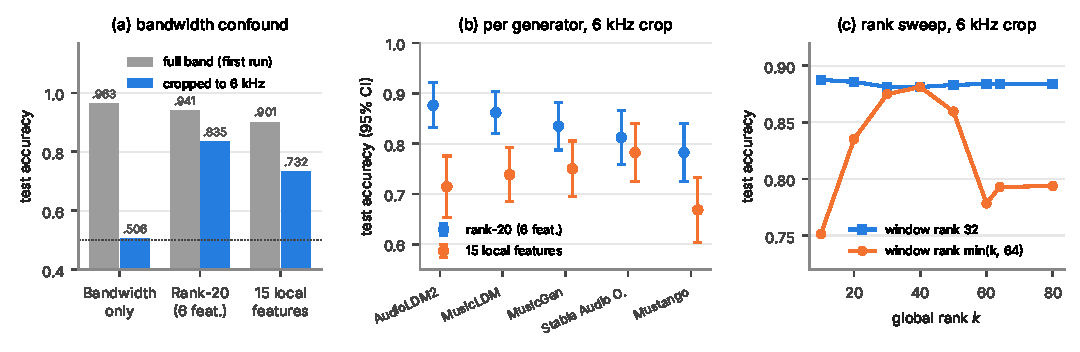
\includegraphics[width=\linewidth]{fig_results.pdf}
\caption{First results (exact per-clip SVD, logistic regression, test split).
(a) Accuracy before and after cropping to 6~kHz; the dotted line is chance.
(b) Accuracy for each generator against its paired human clips, with 95\%
binomial intervals. (c) Accuracy against the global rank $k$ when the window
rank of the principal angles follows $k$ (capped at the window width $w=64$)
and when it is fixed at 32.}
\label{fig:results}
\end{figure}

\begin{table}[h]
\centering\small
\caption{Test accuracy / ROC-AUC. ``Rank-20'' uses six features (top-20
energy, $\sigma_1/\|L\|_F$, effective rank, mean and standard deviation of
principal angles, stability) from the exact SVD with $k=20$; the
15-feature model adds $\sigma_i/\sigma_1$, $i\le8$, and spectral entropy.}
\label{tab:main}
\begin{tabular}{lcc}
\toprule
Model & Full band (first run) & Cropped to 6 kHz \\
\midrule
Bandwidth only (on the processed spectrogram) & --- & 0.506 / 0.513 \\
Bandwidth only (on the raw audio) & 0.963 / 0.933 & \emph{not comparable} \\
Rank-20, exact SVD & 0.941 / 0.980 & 0.835 / 0.923 \\
15 local features, exact SVD & 0.901 / 0.956 & 0.732 / 0.825 \\
15 local + 2 shared-basis features & 0.901 / 0.956 & 0.739 / 0.830 \\
\bottomrule
\end{tabular}
\end{table}

\textbf{The confound and its fix.} All FakeMusicCaps audio was generated at
16~kHz, so it has no content above 8~kHz, while the median human clip reaches
about 15.75~kHz. Our 7~kHz low-pass filter is gentle (about $-7$~dB at 8~kHz),
so the difference survived preprocessing, and a single threshold on bandwidth
separated the classes with 96\% accuracy (Table~\ref{tab:main} and Figure~\ref{fig:results}a). Keeping
only the rows up to 6~kHz removes it: a bandwidth threshold measured on the
processed spectrogram is now at chance for every generator (0.50--0.51). The
SVD features lose about 10 points but stay far above chance, so most of
their signal is not bandwidth. As a further check, we removed every pair with
a raw-audio bandwidth below 6~kHz (519 of 555 test pairs remain): rank-20
accuracy did not change (0.835).

\textbf{Low rank.} AI clips are lower-rank than human ones: mean top-20 energy
0.866 against 0.834, and median effective rank 164 against 177. The effective
rank, however, adds little beyond the top-$k$ energy and the angle features: a
control run with a library randomized SVD per clip, whose effective rank sees
only the top 20 values and is therefore capped at 20, gave the same accuracy
(0.849).


\textbf{Which rank matters.} When the window rank follows the global rank,
accuracy rises from 0.75 at $k=10$ to 0.88 at $k=30$--$40$ and falls to
0.78--0.79 for $k\ge60$ (Figure~\ref{fig:results}c, orange). With the window rank
fixed at 32, accuracy is flat at 0.88--0.89 (AUC $\approx0.95$) for every
global rank from 10 to 80 (blue). So both the rise and the fall come from the
principal-angle features: a window rank of about 30--40 of the $w=64$ frames
works best, and a global rank of 10 is then enough. Our explanation for the
fall, not yet tested, is that as $r\to w$ the window basis spans almost the
whole column space of the window, and with 32 shared frames many angles
between neighbours become zero.

\textbf{Per generator} (Figure~\ref{fig:results}b). The models are trained on all generators and tested on
each generator's clips with their paired human clips (101--130 test pairs,
$\pm0.04$--$0.06$). Rank-20 accuracy is 0.88 for audioldm2, 0.86 MusicLDM,
0.83 MusicGen, 0.81 Stable Audio Open and 0.78 Mustango, the hardest (only 70\%
of its clips are detected as AI). Mustango is also the hardest for the
15-feature model (0.67).

\section{Comparison with a library routine}\label{sec:library}
\textbf{What we compare.} For $N\in\{10,25,50,100,200\}$ training clips
(balanced between the classes) we stack $A=[L_1\cdots L_N]\in\mathbb{R}^{279\times858N}$
and compute (i) the exact thin SVD with NumPy/LAPACK (the reference), (ii)
our randomized SVD with $k=20$, $p=10$ and $q\in\{0,1,2\}$, and (iii)
the scikit-learn randomized SVD with the same $k,p,q$. We record the
criterion from interim report~1,
$\|\tilde\sigma-\sigma\|_2/\|\sigma\|_2\le10^{-2}$ for the leading 20 values, the
per-index errors $|\tilde\sigma_i-\sigma_i|/\sigma_i$, the largest principal
angle between the exact and approximate rank-20 left singular subspaces, and
the median wall-clock time of three runs.

\textbf{Predicted cost.} For a short-and-wide $A$ ($F\ll T$) the thin SVD costs
about $4F^2T$ flops, and the randomized SVD about $2(2q+2)FT\ell$. Both grow
linearly with $T$, so the predicted speed-up is a constant,
$2F/((2q+2)\ell)\approx4.7$ for $F=279$, $\ell=30$, $q=1$. Because $F$ is
small, randomization saves mainly memory and passes over the data, not orders
of magnitude in flops.

\begin{figure}[h]
\centering
\IfFileExists{fig_rsvd_vs_exact.pdf}{%
  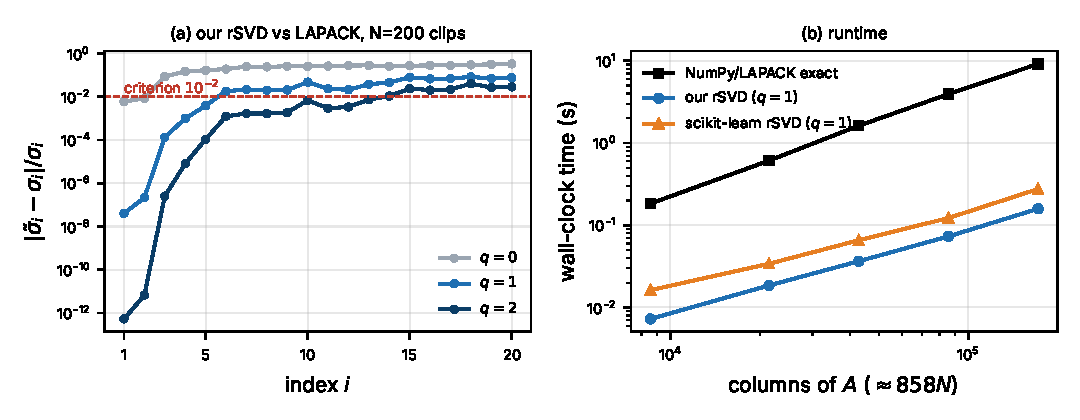
\includegraphics[width=\linewidth]{fig_rsvd_vs_exact.pdf}}{%
  \fbox{\parbox[c][4.2cm][c]{0.9\linewidth}{\centering\small
  % Figure file: fig_rsvd_vs_exact.pdf from the library-comparison run.
  \pending[Figure pending]\\[4pt]
  (a) per-index relative error of our rSVD against LAPACK, $q=0,1,2$, with
  the $10^{-2}$ criterion; (b) wall-clock time against the number of columns
  of $A$ for NumPy/LAPACK, our rSVD and scikit-learn rSVD.}}}
\caption{Our randomized SVD against the exact LAPACK SVD on the stacked
training matrix $A$ ($k=20$, $p=10$; median of three runs). (a) Relative
error of each of the top 20 singular values for $q=0,1,2$ power steps; the
dashed line is the $10^{-2}$ criterion. (b) Wall-clock time against the
number of columns of $A$, $q=1$.}
\label{fig:library}
\end{figure}

\textbf{Results} (Figure~\ref{fig:library}, $N=200$ clips, $A$ of size
$279\times171{,}448$). \emph{Accuracy.} The relative error of the top 20
singular values is $0.072$ with no power step, $0.0116$ with $q=1$ and
$0.0038$ with $q=2$. So $q=1$, the setting planned in interim report~1, misses
the $10^{-2}$ criterion narrowly (0.011--0.016 for every $N$), while $q=2$ meets
it for every $N$ (at most 0.0071). Per index, the errors grow with $i$: with
$q=1$ only $\sigma_1,\dots,\sigma_5$ are within $10^{-2}$, with $q=2$
$\sigma_1,\dots,\sigma_{13}$, and the last values are still off by 2--4\%. This
matches the spectrum: $\sigma_1=9{,}932$ and $\sigma_2=7{,}638$ stand out, but
the tail is flat ($\sigma_{19}=720$, $\sigma_{20}=707$), and the error of a
power-step range finder is governed by ratios $\sigma_{k+1}/\sigma_i$ raised
to the power $2q+1$~\cite{Halko}, which stay close to one here. For the same
reason the largest principal angle between the exact and approximate rank-20
left subspaces stays large (72\textdegree{} for $q=1$, 45\textdegree{} for
$q=2$): directions near index 20 are separated by a gap of only 2\%, so they
are poorly determined by any method, and only the leading directions are
reliable. \emph{Speed.} Exact LAPACK takes 9.2~s; our rSVD takes 0.16~s with
$q=1$ ($58\times$ faster) and 0.23~s with $q=2$ ($40\times$). Runtime grows
linearly in $T$ for our method but faster than linearly for LAPACK (time
$\times50$ for $T\times20$). The measured speed-up is about ten times the
flop-based prediction of 4.7: LAPACK also forms all $171{,}448$ right
singular vectors and is limited by memory traffic, while our method streams
cache-sized $279\times858$ blocks, so flop counts alone do not predict time
here. \emph{Library rSVD.} With the same $k$, $p$, $q$ our implementation has
the same accuracy as scikit-learn's and is 1.7--2 times faster.

\section{What is not working yet, and changes of plan}
\textbf{Not working yet.}
\begin{itemize}\itemsep0pt
\item Our randomized SVD meets the $10^{-2}$ criterion only with two power
  steps, and the singular directions beyond the first few are not reliable
  because the tail of the spectrum is flat (Section~\ref{sec:library}).
\item No bootstrap confidence intervals: every result comes from one test split.
\item The shared-basis features add almost nothing (0.732 to 0.739).
\item Mustango is the weakest generator for both models (AI recall 0.70 and
  0.54); we do not yet know why.
\item The drop in accuracy when the window rank approaches the window width is
  explained only by a hypothesis.
\end{itemize}

\textbf{Changes of plan since interim report 1.}
\begin{itemize}\itemsep0pt
\item \emph{Representation.} Raw magnitude spectrograms with a 2048/512 STFT
  ($1025\times431$) are replaced by mean-subtracted log-magnitude
  spectrograms with a 1024/256 STFT cropped to 6~kHz ($279\times858$). Log
  magnitude follows the feedback on topic; the crop removes the bandwidth
  confound found above.
\item \emph{Data.} Instead of up to 500 pairs we use all 3{,}693 matched
  pairs. The classes are balanced by construction; generators are not
  exactly balanced (700--770 pairs each).
\item \emph{Two power steps.} The stacked-matrix rSVD uses $q=2$ instead of
  $q=1$, because $q=1$ narrowly misses the accuracy criterion.
\item \emph{Two ranks.} The window rank of the principal angles becomes a
  separate parameter from the global rank $k$.
\end{itemize}

\textbf{Interim 1 discussion updates.} The discussion of interim report~1
suggested three directions, which we will start exploring now.
\begin{itemize}\itemsep0pt
\item \emph{Use the singular vectors, not only the singular values.} So far the
  vectors enter only through principal angles. The left vectors $U_k$ show
  \emph{which} frequency patterns carry the energy and the right vectors $V_k$
  show \emph{how} they evolve in time; generators may differ in these shapes
  even when their singular-value profiles are similar, as for Mustango. We will
  start with simple descriptors of $U_k$ and $V_k$ and with class subspaces:
  a human and an AI basis learnt on the training clips with our randomized
  SVD, and a classifier based on the residual of each clip after projection.
\item \emph{Exploit the pairing.} Each AI clip has a human clip with the same
  caption. Listening to paired clips, we found that they are not close
  versions of each other: they are only loosely similar, in instrumentation
  or tonality. The pairing therefore controls the musical content only in part,
  but comparing the two clips should still remove some of the variation due
  to genre and instrumentation. We will start with the principal angles between
  the subspaces of the two clips of a pair and with one SVD of the joint
  matrix $[L_{\rm human}\ L_{\rm AI}]$ per pair, checking how the energy of
  each singular triplet splits between the two blocks of $V$.
\item \emph{Go beyond logistic regression.} A linear model may miss non-linear
  structure, and unsupervised methods show whether the classes separate
  without labels. Following the discussion, we will try linear and RBF SVM and
  $k$-nearest neighbours with the principal-angle distance between clip
  subspaces, which compares the singular vectors directly rather than
  summary features. Without labels, we will run $k$-means with 2 and 6
  clusters on the PCA projection computed with our own SVD, and compare it
  with spectral clustering and an MDS map of the same distances from the
  course labs (adjusted Rand index, purity). Hyperparameters will be tuned on
  the validation split.
\end{itemize}

\textbf{Plan to the final report (21 December).} By 4 December: add bootstrap
intervals and extend the library comparison to larger $N$ and to the accuracy
of the leading singular vectors. By 14 December: singular-vector,
pair-based and classifier experiments, then freeze results. By 21 December:
final report and recording.

\section{Outline of the final report}
\begin{enumerate}\itemsep0pt
\item \emph{Introduction:} AI-music detection, the aim and the scope.
\item \emph{Data and preprocessing:} matching, split, common chain, the
  bandwidth confound and the 6~kHz crop.
\item \emph{Linear-algebra formulation:} the matrix $L$, SVD and
  Eckart--Young, effective rank, principal angles, the stacked matrix $A$.
\item \emph{Algorithms:} exact thin SVD; our randomized SVD (range finder,
  power steps, streaming Gram finish), cost and memory, numerical accuracy.
\item \emph{Library comparison:} error of singular values and subspaces,
  measured time against predicted flops, effect of $q$.
\item \emph{Detection results:} features from singular values and vectors,
  pair-based analyses, classifiers and clustering, bootstrap intervals,
  per-generator results, rank analysis.
\item \emph{Limitations and conclusion.}
\end{enumerate}

\bodyend

\clearpage
\begin{thebibliography}{9}
\bibitem{FakeMusicCaps}
L. Comanducci, P. Bestagini and S. Tubaro,
``FakeMusicCaps: A Dataset for Detection and Attribution of Synthetic Music
Generated via Text-to-Music Models,'' \emph{Journal of Imaging}, vol. 11,
no. 7, article 242, 2025.
\href{https://doi.org/10.3390/jimaging11070242}{doi:10.3390/jimaging11070242}.

\bibitem{Halko}
N. Halko, P. G. Martinsson and J. A. Tropp,
``Finding Structure with Randomness: Probabilistic Algorithms for Constructing
Approximate Matrix Decompositions,'' \emph{SIAM Review}, vol. 53, no. 2,
pp. 217--288, 2011.
\href{https://doi.org/10.1137/090771806}{doi:10.1137/090771806}.

\bibitem{RoyVetterli}
O. Roy and M. Vetterli,
``The effective rank: A measure of effective dimensionality,'' in
\emph{Proc. 15th European Signal Processing Conference (EUSIPCO)},
pp. 606--610, 2007.
\end{thebibliography}

\end{document}
